\documentclass[11pt]{article}
\usepackage[margin=1in]{geometry}
\usepackage{graphicx,booktabs,amsmath,hyperref,natbib}
\title{SDSS Night-Sky Residual Quality Audit}
\author{Biswajit Jana}
\date{\today}
\begin{document}
\maketitle

\begin{abstract}
This is a bounded, reproducible quality-assurance audit of released SDSS
DR17 optical spectra: whether known night-sky wavelength regions
([OI]~5577\,\AA, Na~D~5890\,\AA, [OI]~6300/6364\,\AA, the OH airglow-forest
onset near 7600\,\AA) show elevated uncertainty-normalised residual
structure, $(flux-continuum)\times\sqrt{ivar}$, relative to matched local
control windows of identical width. It is an archive-level QA audit, not a
new sky-subtraction pipeline. The synthetic injection-recovery validation
gate (Section~\ref{sec:validation}) passed: a known 3$\times$ noise-scale
excess injected into the [OI]~5577 window recovered as a median sky/control
residual-scale ratio of 3.87 across 10 synthetic spectra (demo numbers,
Section~\ref{sec:results}), while a shifted-window null test with no
injected line produced a median ratio of 0.86, consistent with no excess.
Fifteen real SDSS DR17 spectra (plate 266, MJD 51630, class-diverse
GALAXY/STAR/QSO sample, deterministic \texttt{SpecObj} query) were fetched
and analysed as described in Section~\ref{sec:data}. The real-data run found
a median sky/control residual-scale ratio of 1.71 (bootstrap 68\% CI
[1.32, 1.83], $n=15$) at [OI]~5577\,\AA\ and 1.95 (CI [1.73, 2.47], $n=13$)
at [OI]~6300\,\AA, both clearly elevated above the no-excess expectation of
1.0, while Na~D~5890 (1.06, CI [1.00, 1.22], $n=15$), [OI]~6364 (0.98, CI
[0.90, 1.11], $n=13$) and the OH-forest onset near 7600\,\AA\ (1.07, CI
[0.98, 1.21], $n=12$) show no comparable excess in this small sample. See
Section~\ref{sec:results} for the full per-window real-data table.
\end{abstract}

\section{Scientific question}
Do known night-sky wavelength regions show elevated uncertainty-normalised
residual structure relative to matched local control windows?

\section{Data and provenance}
\label{sec:data}
Real access uses \texttt{astroquery.sdss.SDSS} (astroquery 0.4.7):
\texttt{query\_sql} runs a deterministic SELECT against the DR17
\texttt{SpecObj} table (\texttt{zWarning=0}, \texttt{snMedian>2}, class in
GALAXY/STAR/QSO, \texttt{ORDER BY specobjid}, \texttt{TOP N}), then
\texttt{SDSS.get\_spectra(matches=...)} downloads each spectrum's
\texttt{spec-*.fits} coadd product. SDSS DR17 is an openly public data
release requiring only acknowledgement of SDSS
\citep{SDSSDr17SpectroBasics}; no login or paywall applies to the CasJobs
SQL or spectrum-download endpoints used here. The real download, when run,
requires explicit operator authorization
(\texttt{scripts/fetch\_data.py --i-have-authorization}). Exact product IDs
(\texttt{spec-PLATE-MJD-FIBER}), retrieval UTC and SHA-256 checksums are
recorded in \texttt{data/manifest.csv}; raw FITS files are not committed.

\section{Method}
For each spectrum, wavelength is the vacuum Angstrom value
$10^{\mathrm{loglam}}$ from the HDU1 COADD table
\citep{SDSSSpecDatamodel}. A low-order (degree-1), inverse-variance-weighted
polynomial continuum (\texttt{continuum.py}, normalised wavelength axis to
avoid ill-conditioning) is fit to a baseline region surrounding but
excluding each documented night-sky window and its matched local control
window of identical width (\texttt{windows.py}). Per-pixel
uncertainty-normalised residuals
$r_i = (\mathrm{flux}_i-\mathrm{continuum}_i)\sqrt{\mathrm{ivar}_i}$
(\texttt{residuals.py}) are aggregated per window into a robust
(1.4826$\times$MAD) scale statistic. \texttt{metrics.py} computes the
sky-vs-control excess statistic per spectrum per window pair: the ratio and
difference of the sky-window scale to the control-window scale. SPPIXMASK
bit definitions were verified live against the SDSS DR17 bitmask
documentation \citep{SDSSDr17Bitmasks}, which itself names 5577\,\AA\ as a
wavelength where pipeline error estimates ``can be untrustworthy'' --- a
documented, not invented, motivation for this audit. The four
sky-residual-quality bits (NOSKY, BRIGHTSKY, BADSKYCHI, REDMONSTER) are
deliberately \emph{not} excluded by the default good-pixel mask, since they
are partly the phenomenon under study; \texttt{masks.py} exposes them
separately for the mask-sensitivity check. Night-sky line centre
wavelengths follow the commonly quoted values covered by the flux-calibrated
optical sky atlas of \citet{Hanuschik2003SkyAtlas}, documented in
\texttt{docs/ASSUMPTIONS\_AND\_LIMITATIONS.md} rather than claimed as
atlas-precision measurements. Results are aggregated across spectra
(median), bootstrapped for uncertainty, and stratified by SDSS object class
and \texttt{snMedian}-derived SNR bins (\texttt{metrics.py}).

\section{Validation and uncertainty}
\label{sec:validation}
Observational uncertainty is bootstrap-resampled (1000 resamples, seed
20260713, \texttt{bootstrap.bootstrap\_statistic}); numerical convergence of
each continuum fit is assessed separately via covariance conditioning and
reduced $\chi^2$ (\texttt{bootstrap.check\_fit\_convergence}), never
conflated with the bootstrap interval.

The required synthetic injection-recovery gate
(\texttt{tests/test\_core\_pipeline.py}) injects a known 3$\times$ noise-scale
excess into the [OI]~5577 sky window of 10 synthetic spectra
(\texttt{synthetic.py}) and confirms \texttt{run\_pipeline} recovers an
elevated sky/control residual-scale ratio there. In the demo run reported
here, the median recovered ratio was 3.87 ($n=10$ spectra), consistent with
the injected 3$\times$ excess (residual-scale ratios are not expected to
equal the injected sigma-scale factor exactly, since scale statistics
combine injected and base noise nonlinearly). \textbf{This gate passed.} A
shifted-window null test (\texttt{null\_tests.py}) compares two
control-style windows against each other, neither coincident with a
documented sky line; the demo run's median null ratio was 0.86, within the
tolerance of 1.0 expected for no true excess. A mask-sensitivity check
(rerunning with \texttt{extra\_exclude\_bits=SKY\_QUALITY\_BITS}) and
class/SNR stratification are both exercised in the test suite
(\texttt{tests/test\_masks.py}, \texttt{tests/test\_metrics.py}).

\section{Results}
\label{sec:results}
All numbers below are read directly from \texttt{results/summary.json}.

\textbf{Demo (synthetic) run:} \texttt{scripts/run\_analysis.py --demo}
generates 10 synthetic spectra with a known 3$\times$ excess injected into
the [OI]~5577 window. Median sky/control residual-scale ratio for the
injected window: 3.87 ($n=10$). Shifted-window null test median ratio:
0.86 ($n=10$), consistent with no excess where none was injected. These are
clearly-labelled synthetic smoke-test numbers, not real SDSS measurements
(\texttt{data\_kind: "synthetic\_demo"} in \texttt{results/summary.json}).

\textbf{Real-data run:} \texttt{data\_kind: "real public SDSS spectra"} in
\texttt{results/summary.json}, 15 spectra fetched (plate 266, MJD 51630;
\texttt{data/manifest.csv} has the full product-ID/checksum list), all 15
successfully processed by \texttt{run\_pipeline} (\texttt{n\_spectra\_used =
15}). Per-window median sky/control residual-scale ratio and bootstrap 68\%
confidence interval (1000 resamples, seed 20260713):
\begin{center}
\begin{tabular}{lccc}
\toprule
Window & $n$ & median ratio & 68\% CI \\
\midrule
{[OI]}~5577 & 15 & 1.711 & [1.325, 1.829] \\
Na~D~5890 & 15 & 1.059 & [1.005, 1.216] \\
{[OI]}~6300 & 13 & 1.949 & [1.733, 2.474] \\
{[OI]}~6364 & 13 & 0.984 & [0.905, 1.114] \\
OH forest onset ($\sim$7600) & 12 & 1.070 & [0.979, 1.207] \\
\bottomrule
\end{tabular}
\end{center}
Both auroral [OI] windows (5577 and 6300\,\AA) show a bootstrap CI that
excludes 1.0, i.e.\ elevated uncertainty-normalised residual structure
relative to their matched local control windows in this real, small
($n\le15$) sample. Na~D, [OI]~6364 and the OH-forest onset window do not
show a comparable excess here; sample sizes below 15 reflect spectra for
which that window pair fell outside the observed wavelength range or had
too few good baseline pixels (recorded in \texttt{results/warnings.json},
7 warnings, none causing a full spectrum to be dropped). This is a small,
deterministic sample bounded by the authorized query size, not a
survey-scale claim.

\section{Limitations}
\label{sec:limitations}
A bounded, released-product QA audit; not a new sky-subtraction pipeline,
and not a substitute for the DESI/idlspec2d pipeline internals
\citep{Guy2023DESIPipeline} or the general-purpose \texttt{skycorr} tool
\citep{Noll2014Skycorr}. The continuum estimate is a low-order local
polynomial, not a physically motivated stellar/galaxy/QSO template fit;
genuine astrophysical emission or absorption features coincidentally near a
sky window could bias that spectrum's local continuum estimate and hence
its excess statistic. The real sample is necessarily small (bounded by an
explicit, deterministic SpecObj query), so per-class/per-SNR stratified
results should be read with wide uncertainty in mind; sample sizes are
recorded, not hidden, in \texttt{results/summary.json} and
\texttt{results/warnings.json}. Night-sky line centre wavelengths are
commonly quoted round values, not atlas-precision measurements re-derived
from \citet{Hanuschik2003SkyAtlas}. \texttt{reports/report.tex} could not be
compiled to PDF in this environment (no local LaTeX toolchain); only
structural completeness was verified. See
\texttt{docs/ASSUMPTIONS\_AND\_LIMITATIONS.md} for the full list.

\section{Reproducibility}
\begin{verbatim}
python -m pip install -e ".[dev]"
pytest -q
ruff check .
mypy src
python scripts/run_analysis.py --demo
python scripts/make_figures.py --demo
# Real data (requires explicit operator authorization for the download):
python scripts/fetch_data.py --i-have-authorization
python scripts/run_analysis.py
python scripts/make_figures.py
python scripts/sync_web_assets.py
\end{verbatim}
Software version, git commit and configuration SHA-256 are recorded in
\texttt{results/summary.json} and each figure's sidecar JSON.

\begin{figure}
  \centering
  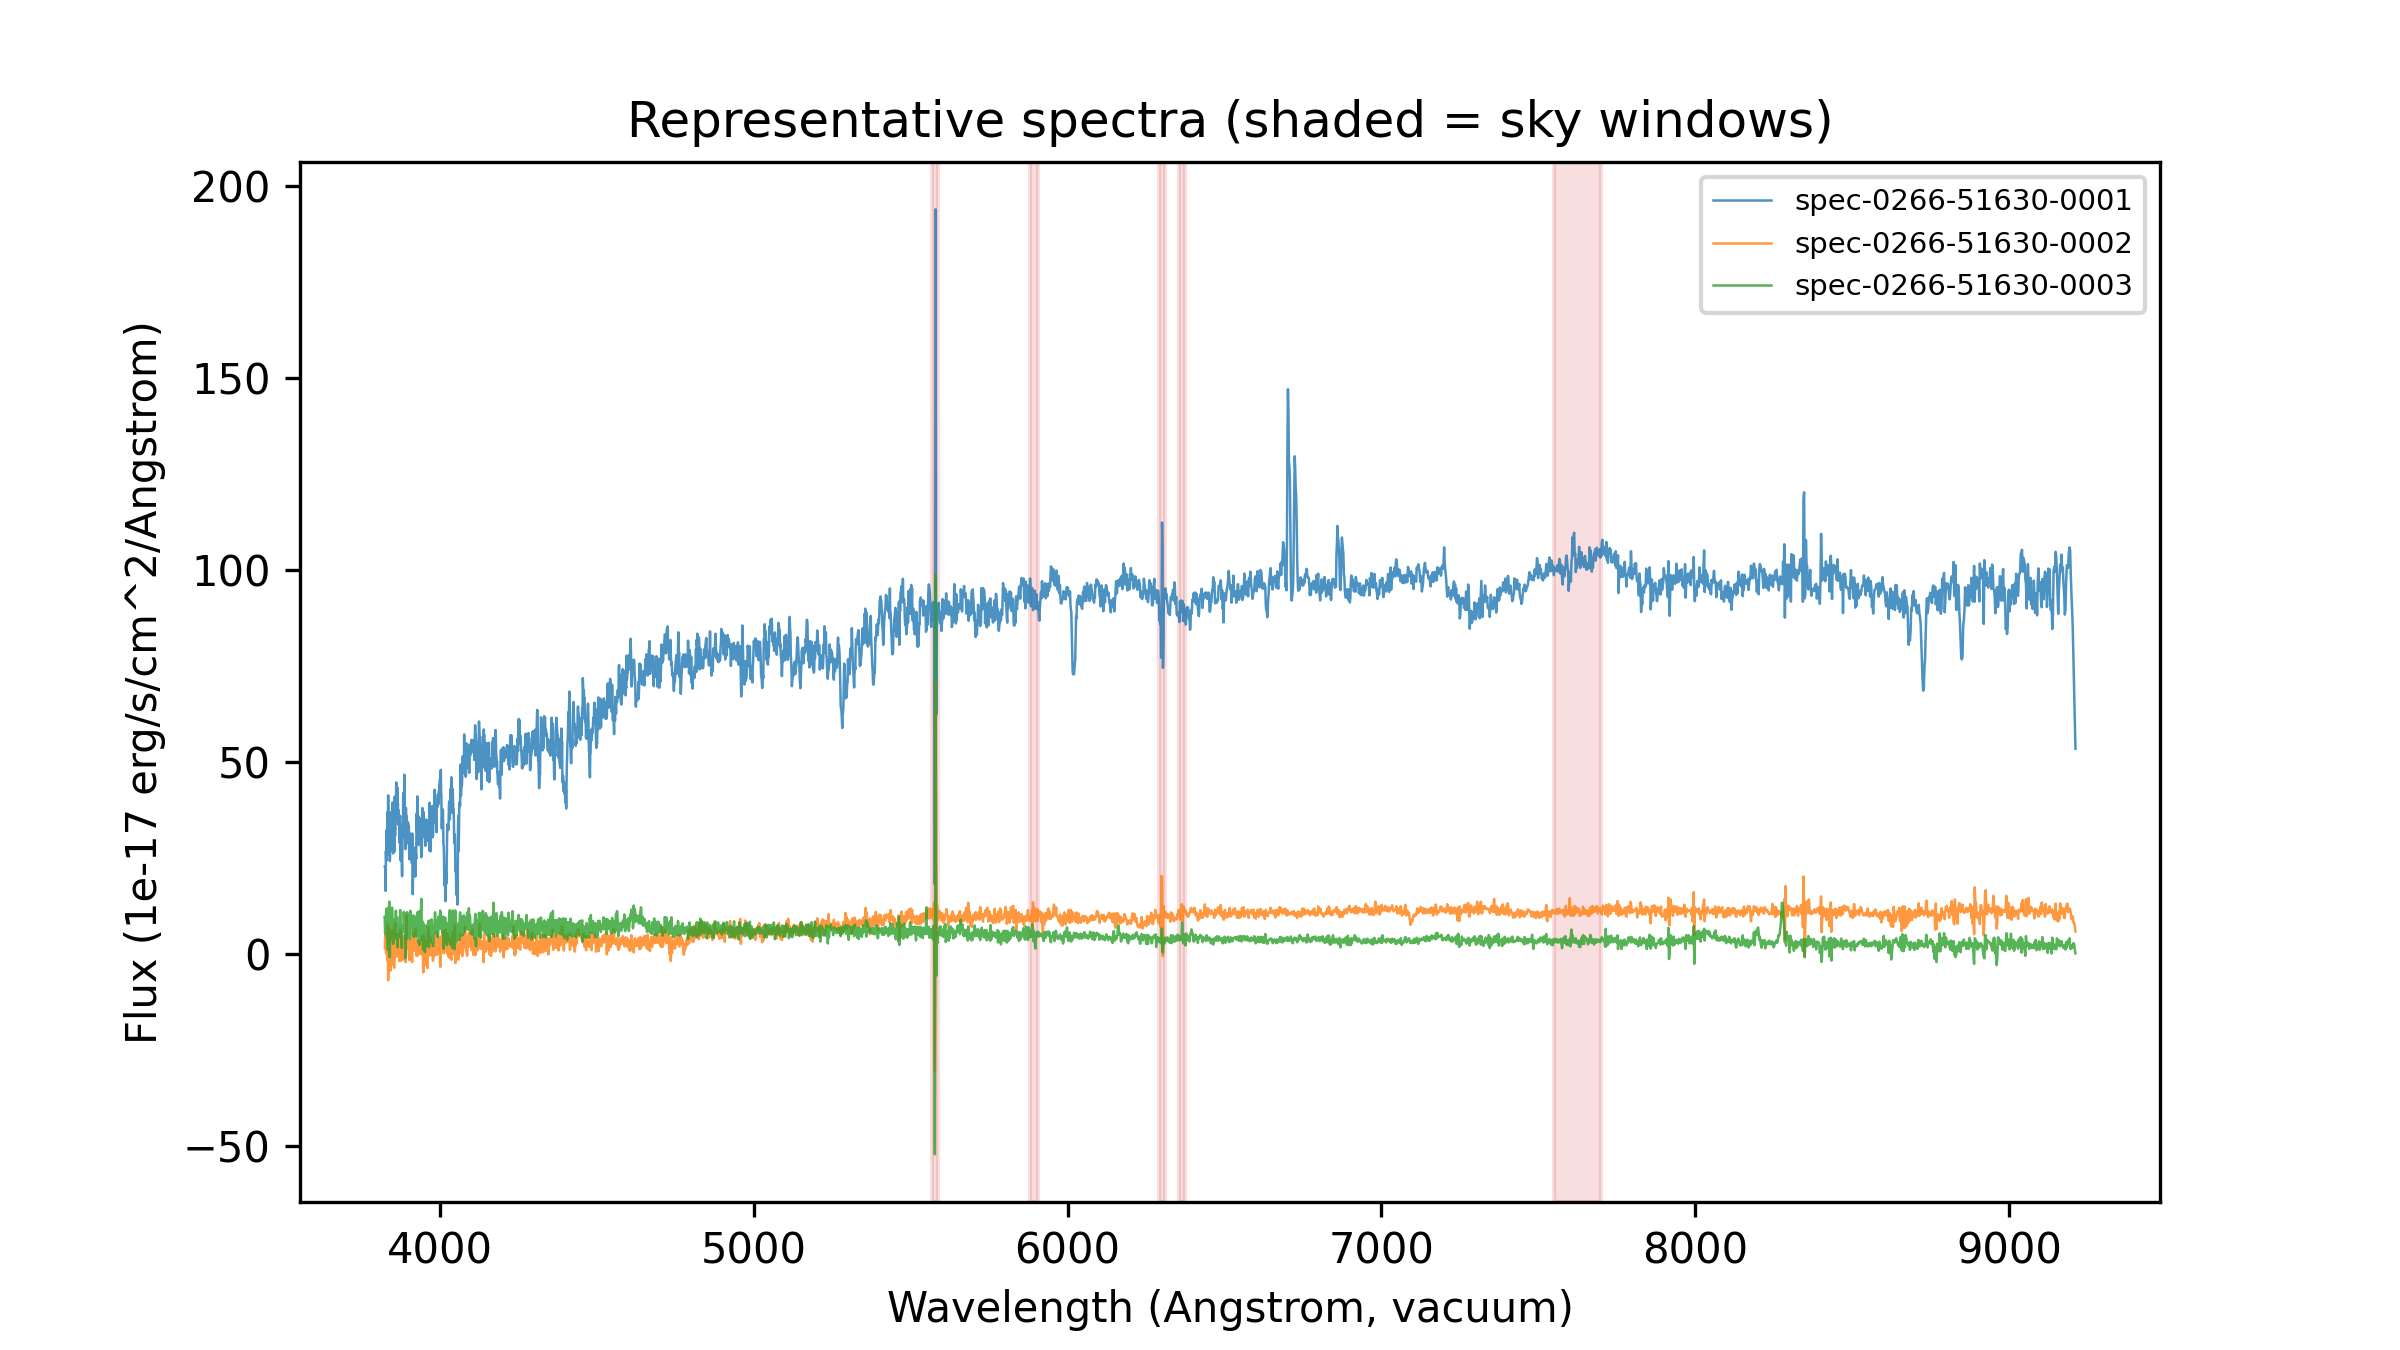
\includegraphics[width=0.7\textwidth]{../figures/fig01_representative_spectra.png}
  \caption{Representative spectra with documented night-sky windows shaded.}
  \label{fig:spectra}
\end{figure}

\begin{figure}
  \centering
  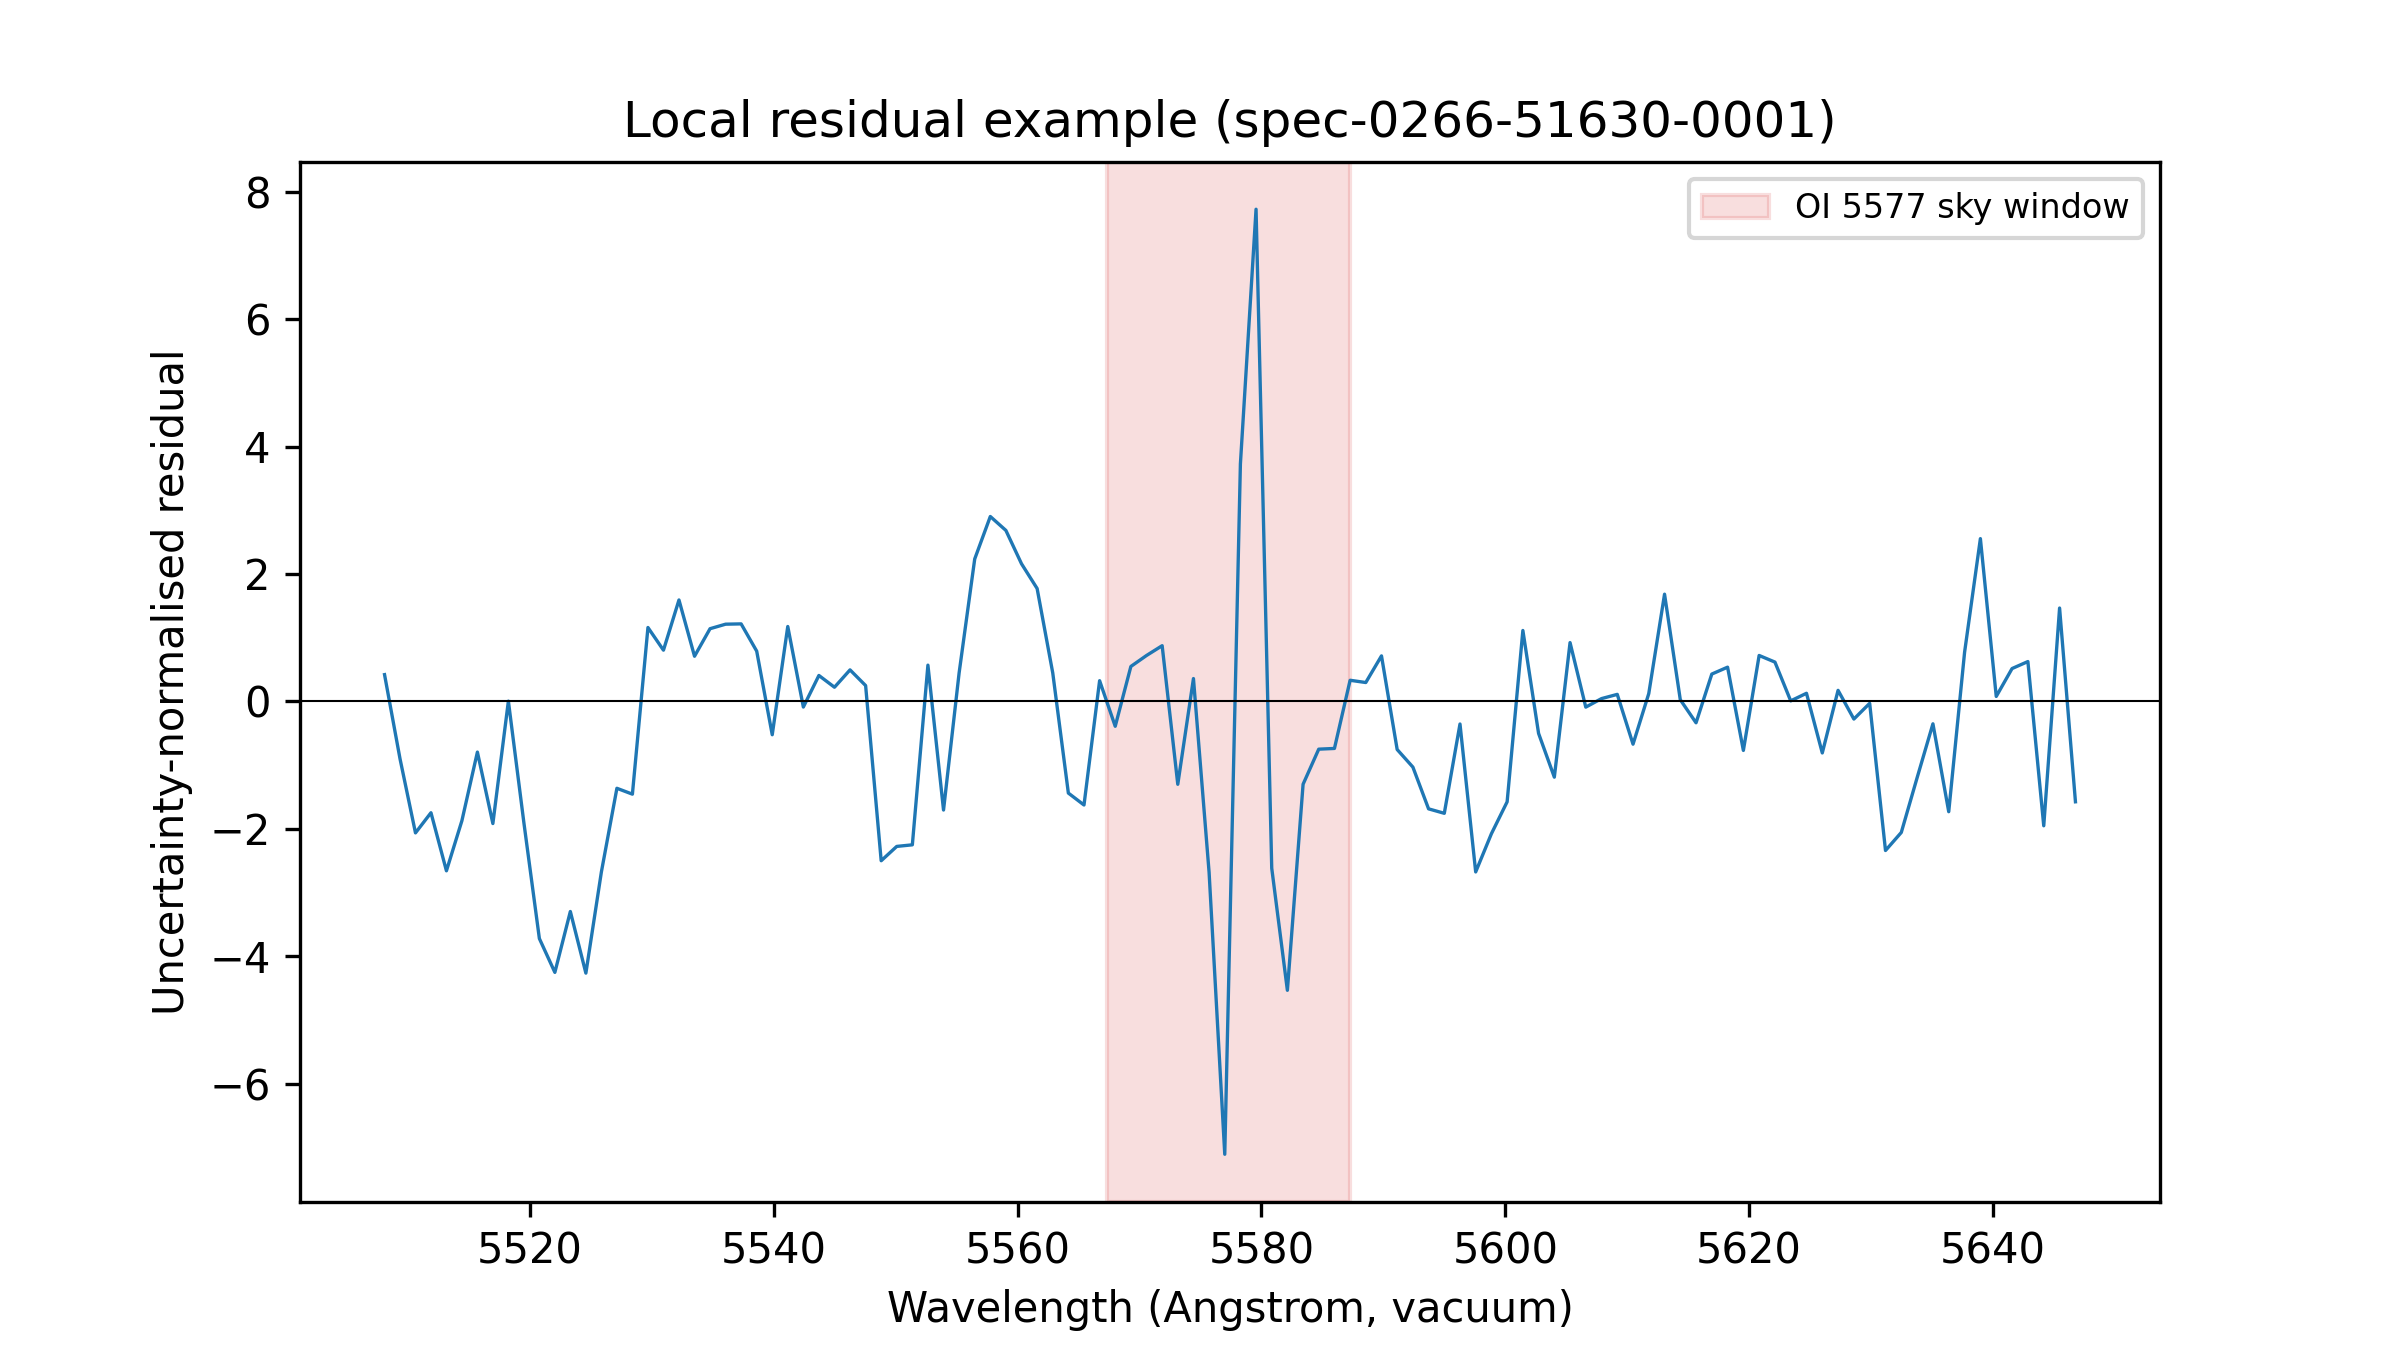
\includegraphics[width=0.7\textwidth]{../figures/fig02_local_residual_example.png}
  \caption{Local uncertainty-normalised residual example around the
  [OI]~5577 sky window for one spectrum.}
  \label{fig:residual}
\end{figure}

\begin{figure}
  \centering
  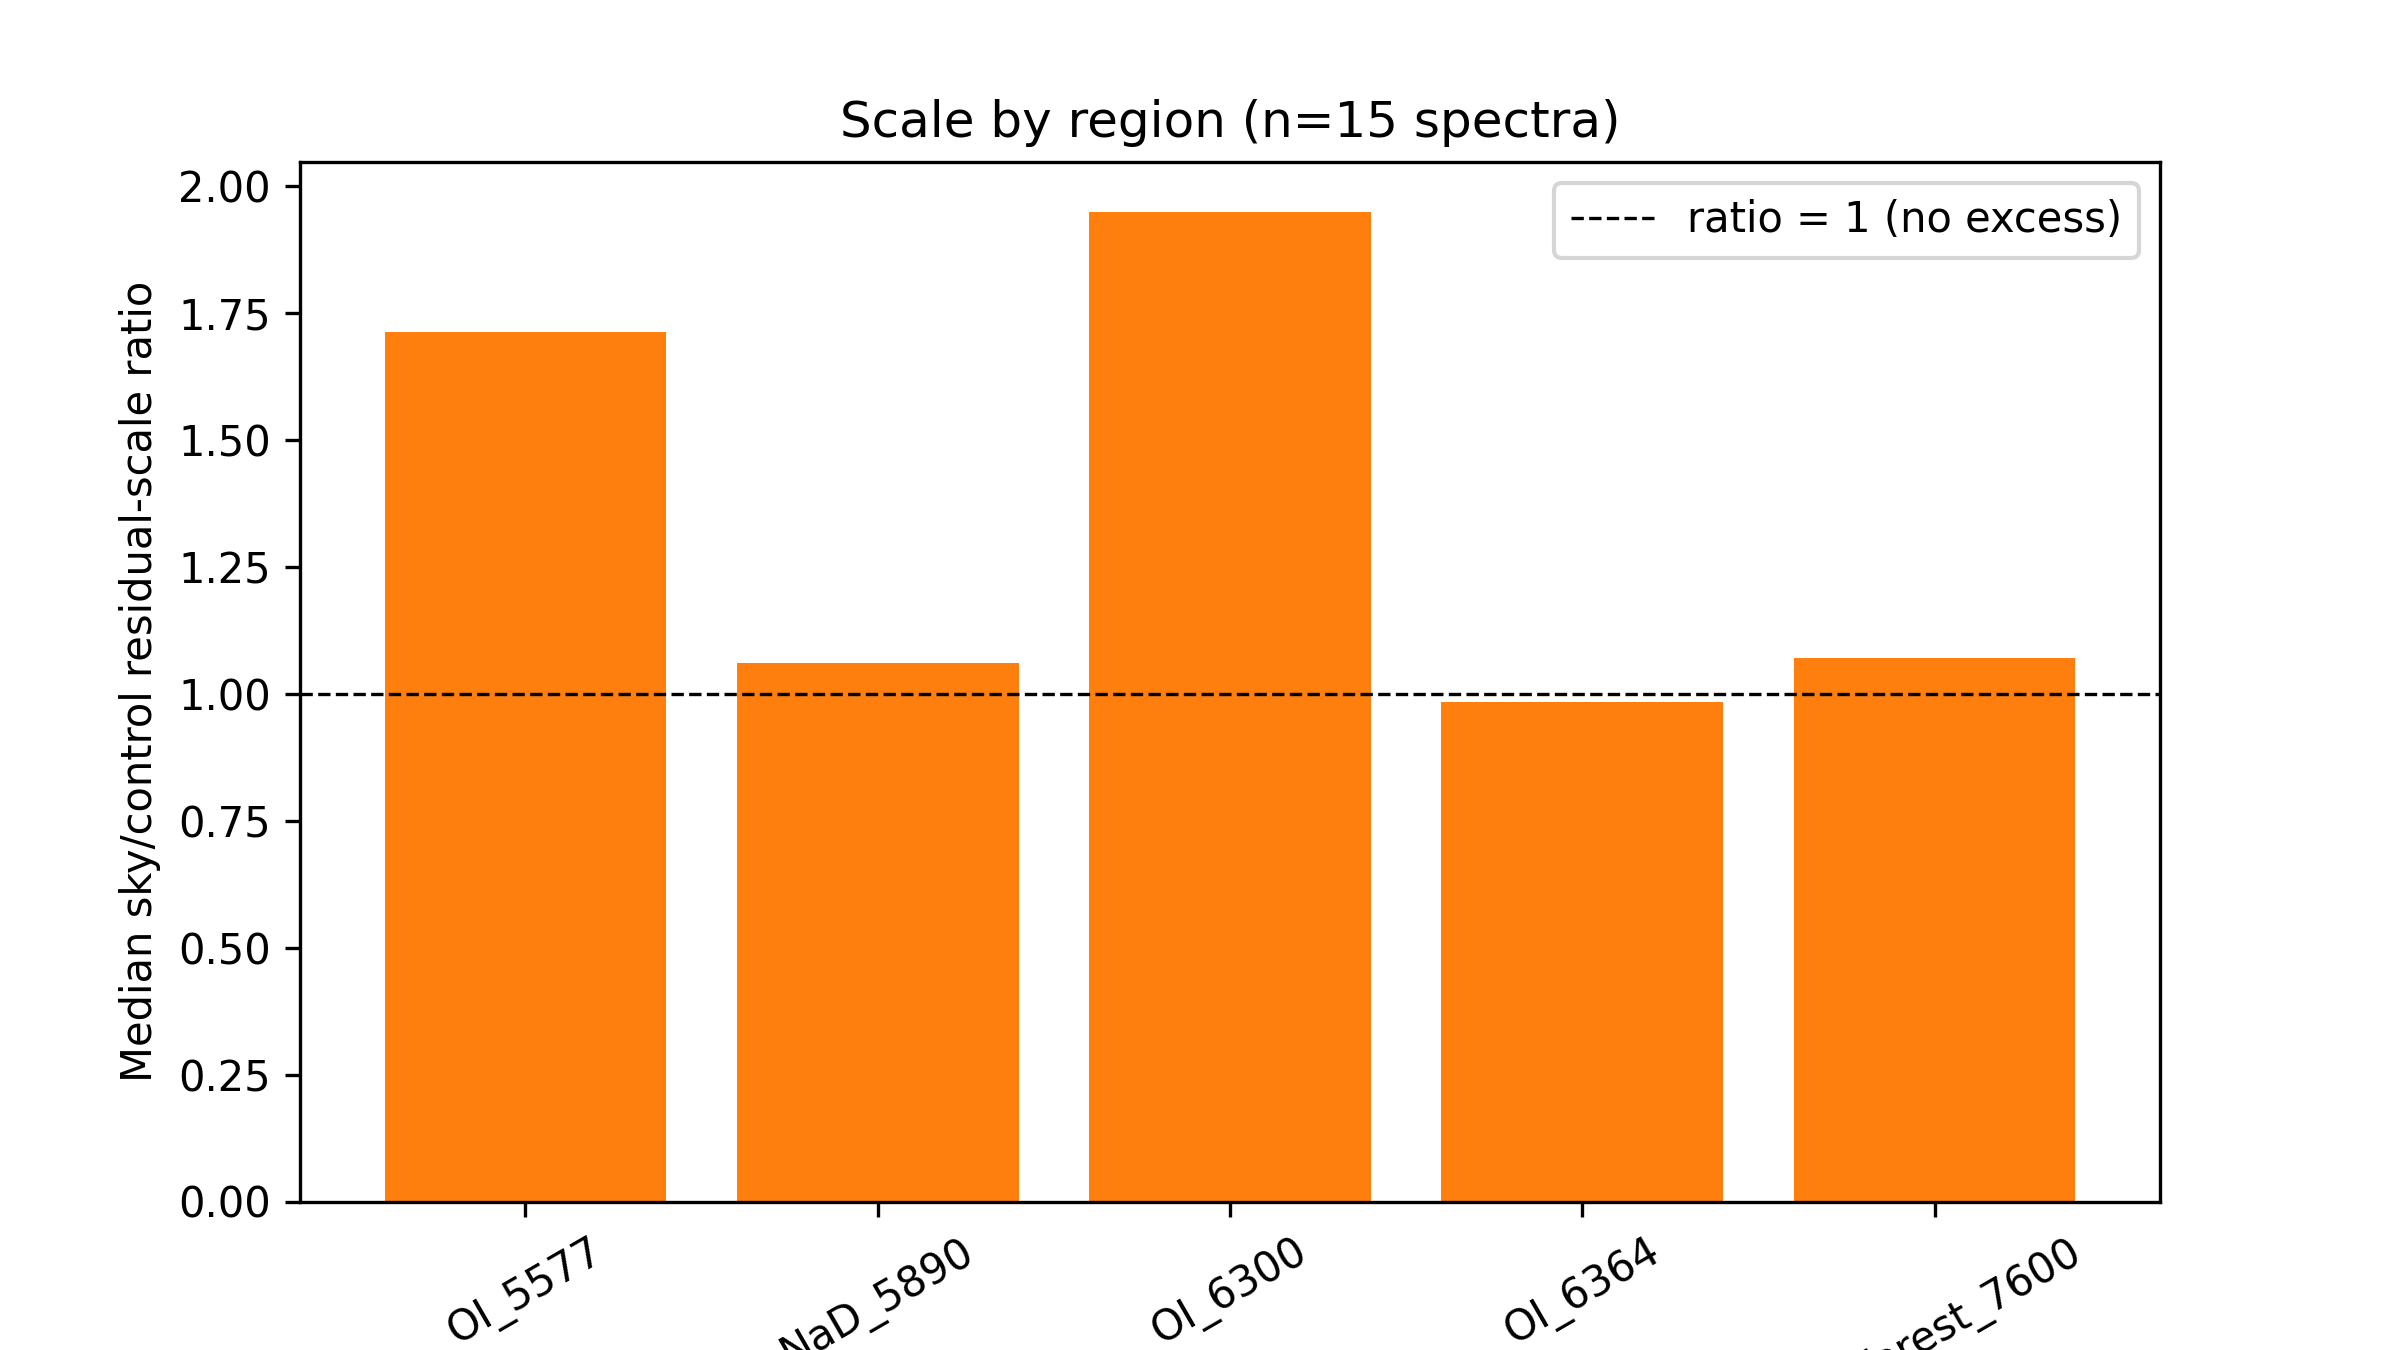
\includegraphics[width=0.7\textwidth]{../figures/fig03_scale_by_region.png}
  \caption{Median sky/control residual-scale ratio by window-pair label.
  Ratio $=1$ indicates no excess.}
  \label{fig:scale}
\end{figure}

\begin{figure}
  \centering
  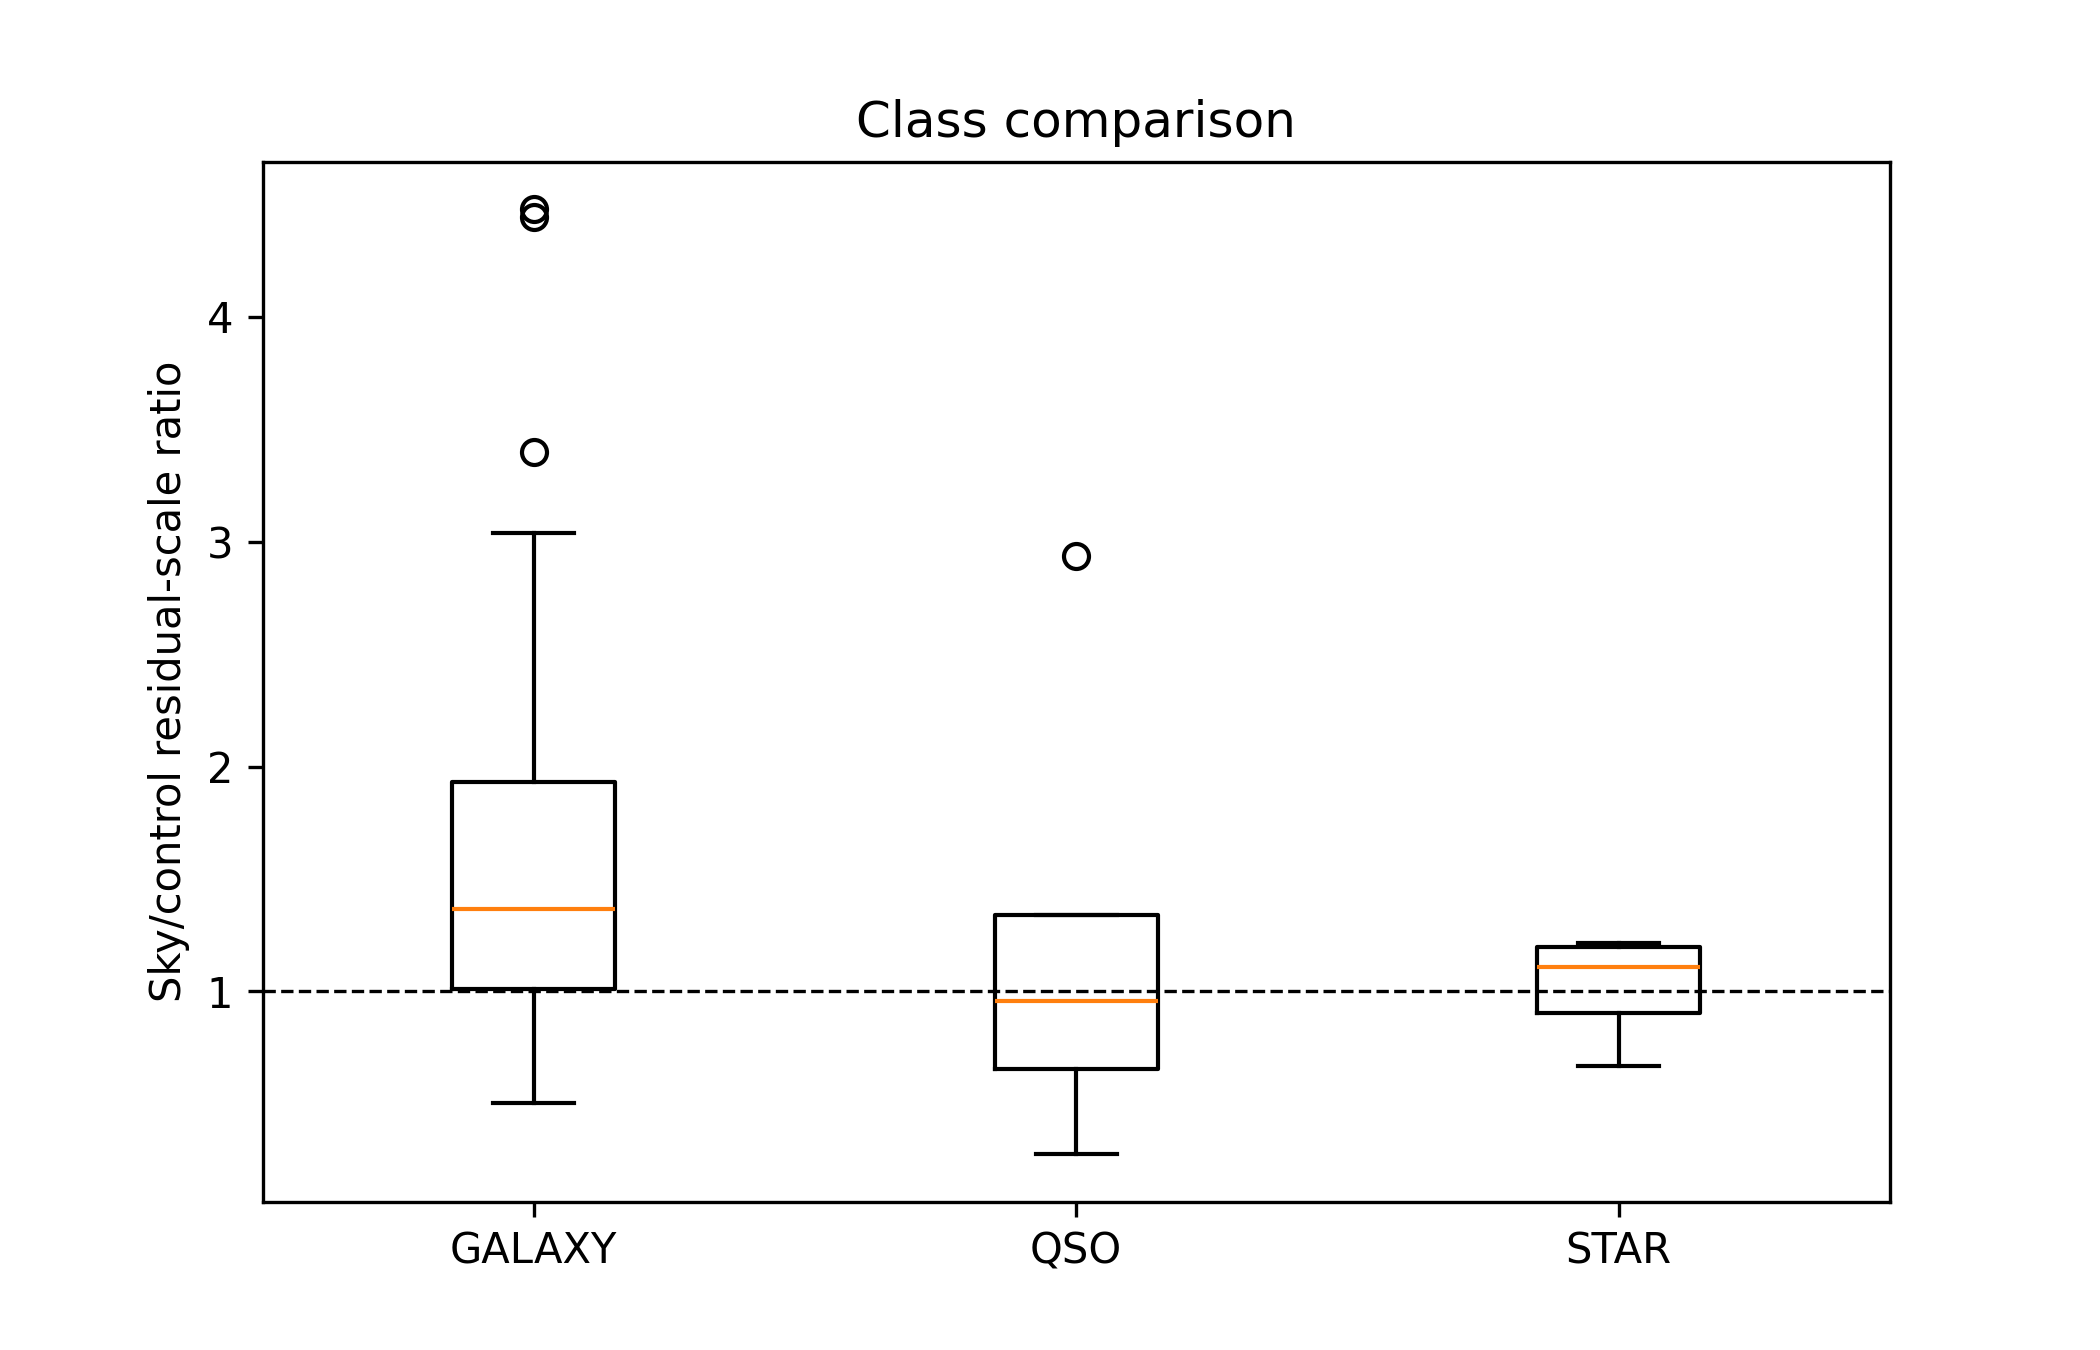
\includegraphics[width=0.6\textwidth]{../figures/fig04_class_comparison.png}
  \caption{Sky/control residual-scale ratio distribution by SDSS object
  class.}
  \label{fig:class}
\end{figure}

\begin{figure}
  \centering
  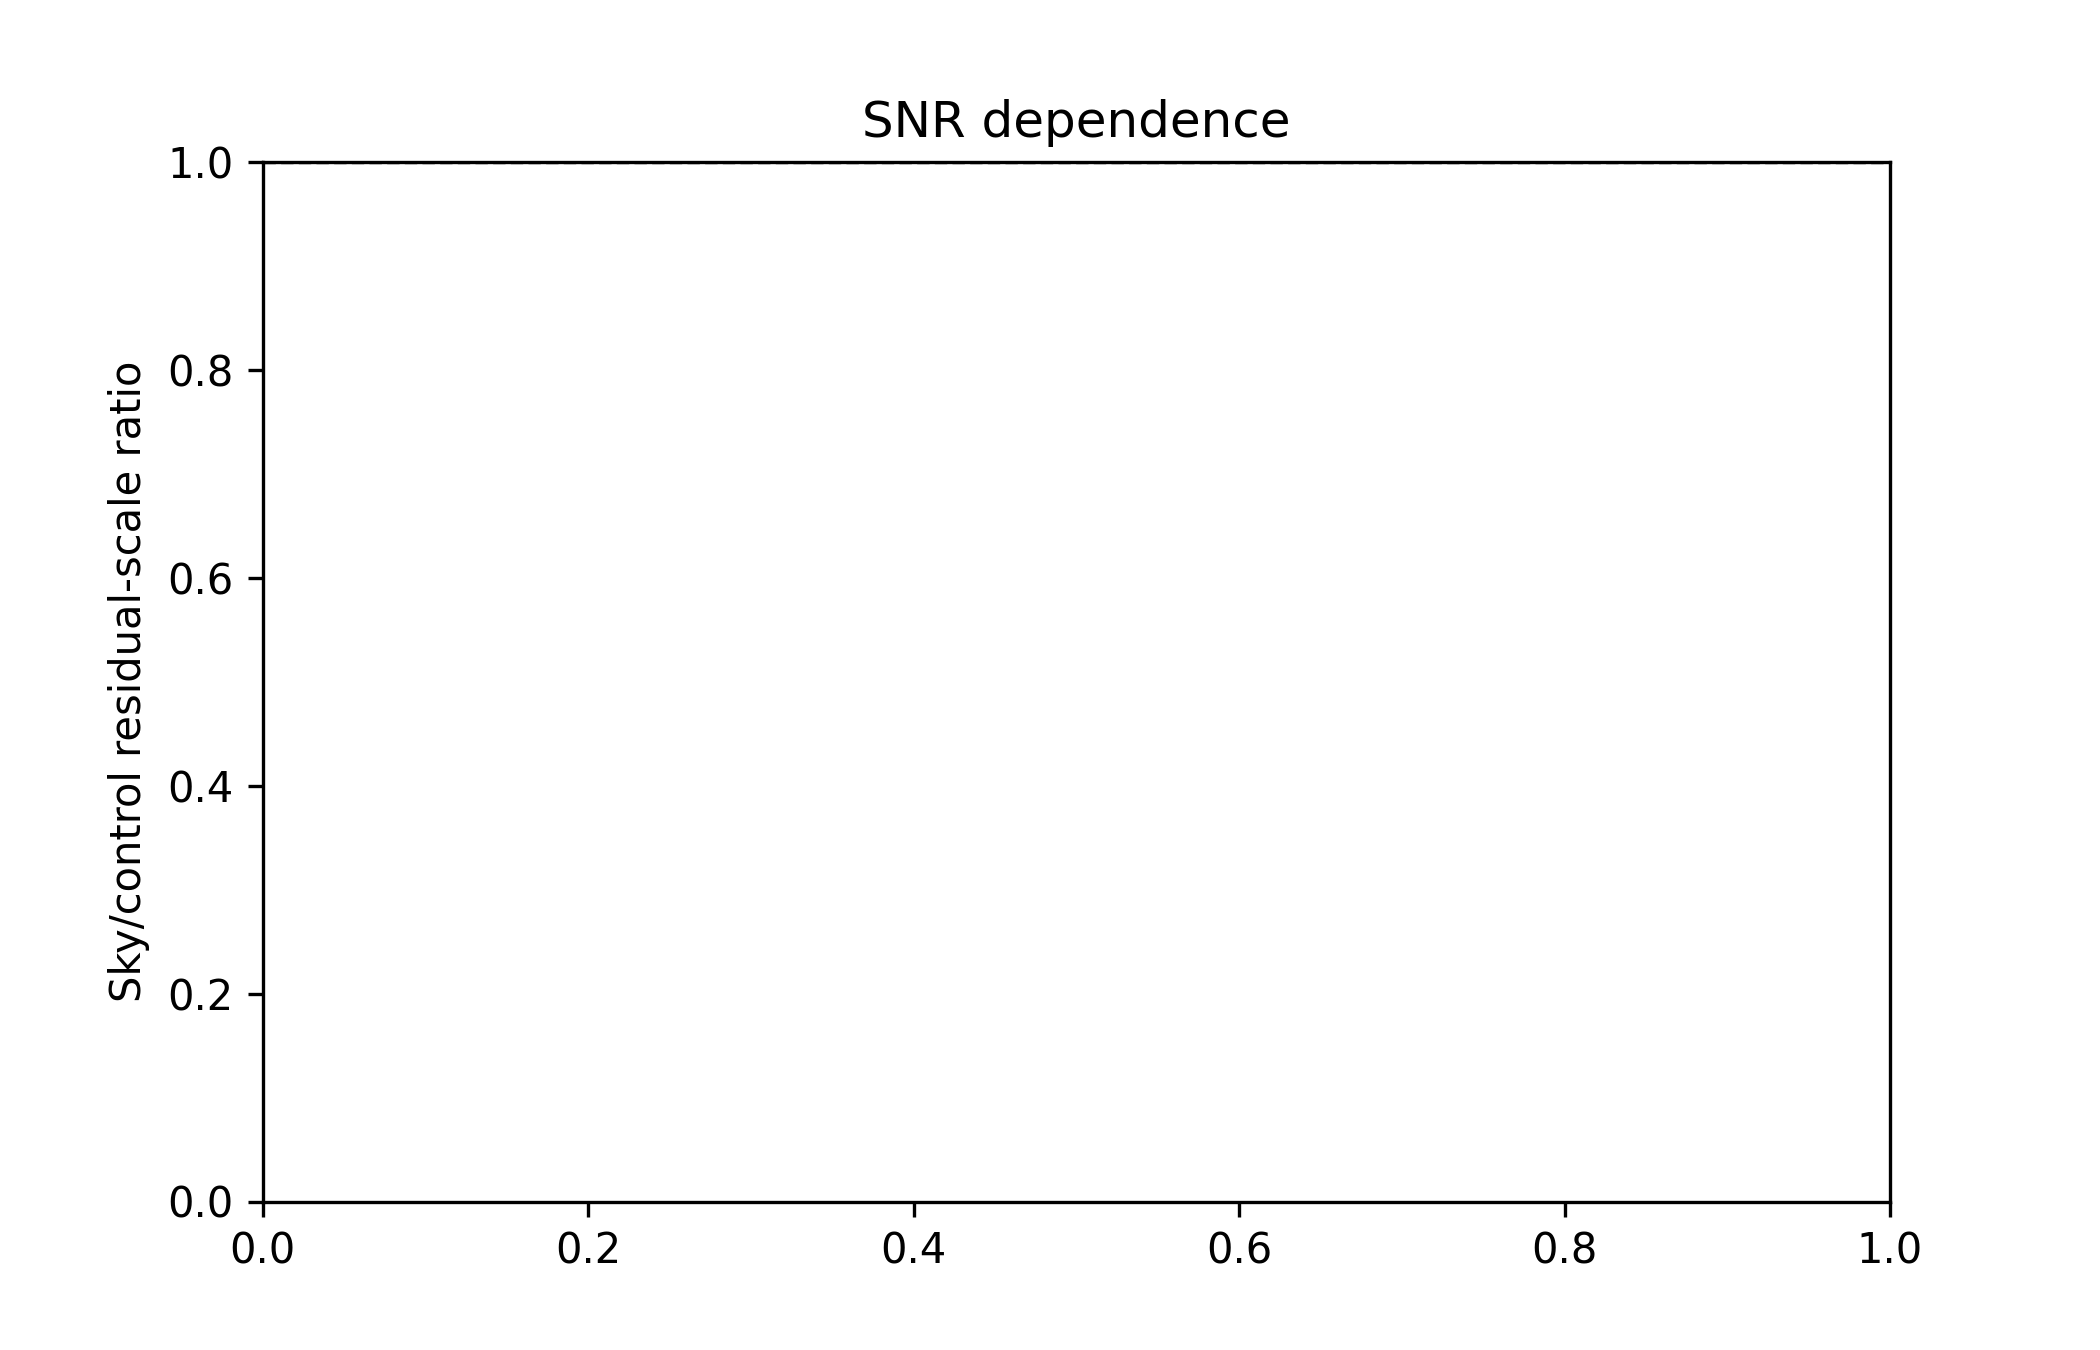
\includegraphics[width=0.6\textwidth]{../figures/fig05_snr_dependence.png}
  \caption{Sky/control residual-scale ratio distribution by S/N bin.}
  \label{fig:snr}
\end{figure}

\begin{figure}
  \centering
  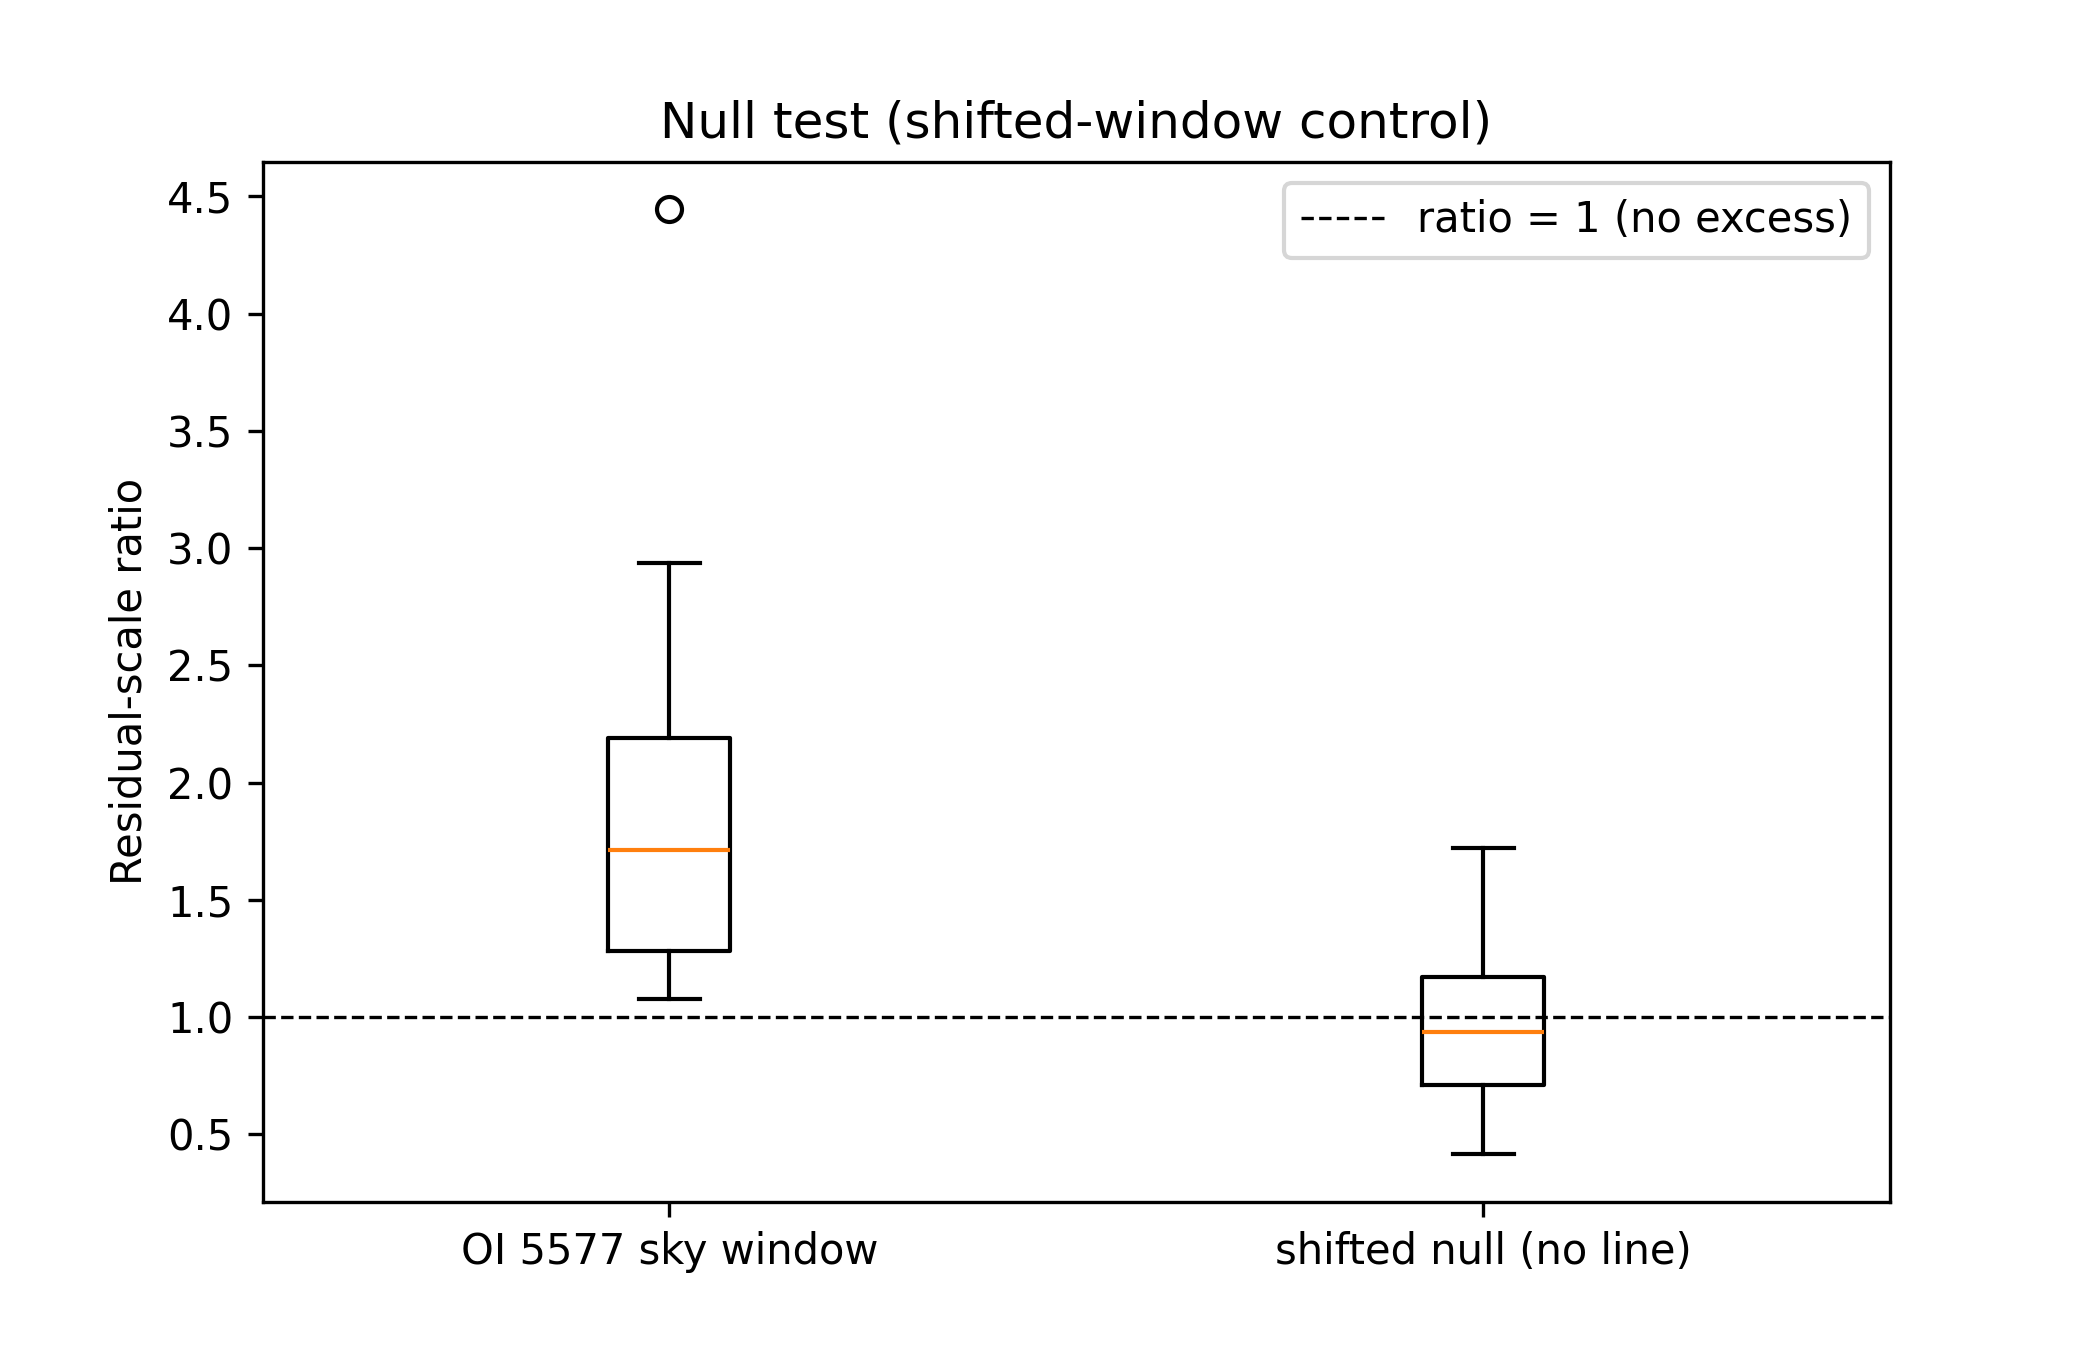
\includegraphics[width=0.6\textwidth]{../figures/fig06_null_test.png}
  \caption{Injected sky-window ratio vs.\ shifted-window null-test ratio
  (Section~\ref{sec:validation}).}
  \label{fig:null}
\end{figure}

\bibliographystyle{plain}
\bibliography{references}
\end{document}
